\documentclass[a4paper, 11pt]{article}

\usepackage[english]{babel}
\usepackage[utf8]{inputenc}
\usepackage[T1]{fontenc}
\usepackage{hyperref}
\usepackage{graphicx}
\usepackage{wrapfig}
\usepackage{float}
\graphicspath{rep\images_latex}

\begin{document}
\title{
  Annotator and Mask recognizer \\
  \large Master 2 at University Of Côte d'Azur
}
\author{Fissore Davide, Galbiati Federica and Venturelli Antoine}
\maketitle
\tableofcontents


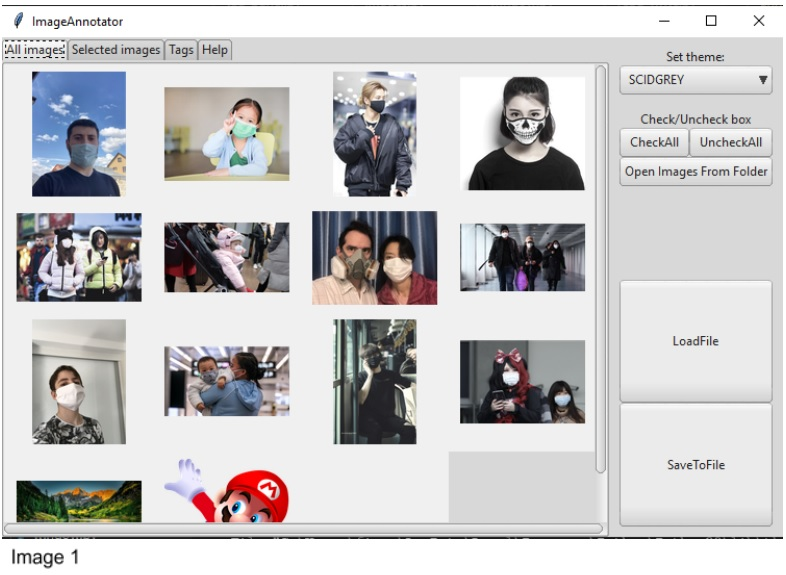
\includegraphics[scale=.6]{images_latex/Image_annotator.jpg}

\section{Overview}
Overview
Programming language Python version 3.9.7 with following libraries :
\begin{itemize}
  \item PIL to load and treat images
  \item tkinter to charge the graphic interface
  \item json to save and load json encoded files
  \item ttkthemes to get a larger library of theme for our interface
  \item tkhtmlview to display simple HTML and CSS text
  \item shapely to work on shapes and get coverage methods
\end{itemize}

\section{How to run the project}
The project can be launched from the src folder (this is mandatory so that imports of local
files go correctly) opening the  \textit{window.py}  file. It  will take few seconds to load all libraries, for
example the ttkthemes import is a bit slow and also the interface will be less reactive, to
avoid this you can pass the  \textit{“-fast”}  optional parameter  to open the classic tk.Tk() window
(exemple  \textit{python3 ./window.py -fast},  note that the  python3 command may not work on
some OS for example in certain windows distributions you should use py).

\section{Task repartition}
We did the most part of the project at University in an available room 
and we collaborated to create together each aspect of the project.
In particular we divided the work as follow:
\begin{itemize}
  \item Antoine worked on the graphic interface, for example, he added the different options such as scrolling menu, notebook or tooltip.
  \item Davide created the class for adding, renaming tags and images and annotation treating.
  \item Federica had deal with the help panel (using HTML and CSS), with the parse and save of JSON files and train different models to find the best. 
\end{itemize}


\section{Project structure}
The project is characterized by four main folders:
\begin{itemize}
  \item src: containing the python file source
  \item img: containing a sample of images that can be used in the program (these images are taken from kaggle)
  \item pre: containing pretreatment scripts (it is still empty)
  \item rep: containing the report of the project
\end{itemize}

\section{Short script description}
In the src folder there are 8 scripts and a text folder in which there are some simple HTML files used for the help menu.
The interface is created via the \textit{window.py} file and it integrates the \textit{tag\_panel} and the \textit{helppanel.py} files.
The \textit{annotator.py} file aims to create a separate window in which it is possible to open an image and add some annotation on it.
Finally, \textit{images.py} and \textit{tags.py} help to store data in images whereas \textit{read\_write.py} and \textit{scrollableframe.py} are useful files to, respectively, read and write JSON files and create scrollable windows within the interface.

\section{Main features (code behind the scene)}
The code is based on two classes that hold the main logic to create annotation on image and tag manipulation.
\subsection{The img class}
The img class takes in paramater the image path and, from it, creates the base attributes needed to store other information such as the \textit{set} of tags ST and the \textit{dict} of association DA {tag: list of coordinates associated to this tag}.
We can create a new association in the DA via the \textit{add\_tag} method taking as parameter the name of tag (if it doesn't exist in out ST it will be added) and the top-left couple and the bottom-right coordinates of the newly-created annotation.
In this method we do some checks to verify if these coordinates are valid: a rectangle is not valid if its \textit{"surface is less than 40 pixels in total or spatial dimensions (heigh and width) are too small, for example less than 5 pixels. Moreover, if a box has an intersection with other boxes for more than 20\% of its surface, it should be discarted.
One should also discard a box if it completely covers a pre-existing box or it is completely contained in a pre-existing one"} (indication from project subject). 
In this class we have other tools to handle annotation removal, tag rename and some methods to create tkinter \textit{Label} containing the desired image for the interface.
Finally the \textit{\_str\_} and \textit{\_repr\_} methods (similar to the toString method in java class) are use to return the string representation of an img object to be printed in a JSON file. 
\subsection{The tag class}
The tag class extends the set type of Python since we do not want any repetition of a pre-existing tag, moreover a tag object owns a list of \textit{imgs} to know every image of our application and perform \textit{side effect} operation if needed.
For example, when we rename tag A in tag B, we take every img from the \textit{imgs} list of our current tag object and, if the image owns A, it will rename it in B. Similar operations are done for removal (every image will pop the tag key from its \textit{dict} of annotation) and insertion.  

\section{Added features (code for the interface)}
\subsection{"All images" and "Selected images" panels} 
Our interface is conceived to cover the wanted functionalities. When we run the project, we can see the first panel shown in image 1 listing all the images of the \textit{img} folder.
Here we can select the sample of images (by clicking on it) that will be available in the \textit{"selected images"} panel for annotation phase. 
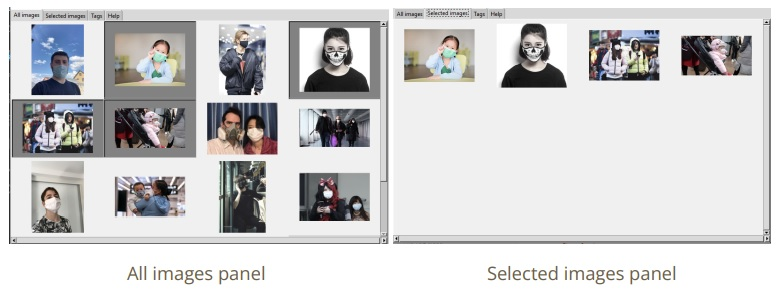
\includegraphics[scale=0.8]{images_latex/images_panel.jpg}
In the selected images panel you can click on the image you want to annotate and the new window will pop up. 
\subsection{The annotator}
\begin{wrapfigure}{l}{0.5\textwidth}
  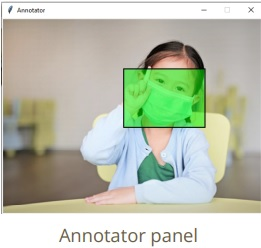
\includegraphics{images_latex/annotator.jpg}
\end{wrapfigure}
Here, you can click a first time to draw the rectangle of the annotation and a second time to draw it (in case of error you can click the \textit{ESC} button of the keyboard to undo the operation).
When the user has confirmed the annotation you will see either the image 2 if you still have no pre-existing tag where you can enter your new tag and save it in the tag set, or the Image 3 which is similar to the Image 2 with the possibility to choose one among the existing tags (Image 4) thanks to an OptionMenu.
\begin{figure}[htb]
  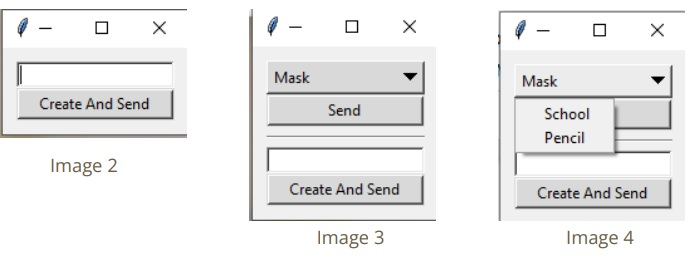
\includegraphics[scale=0.9]{images_latex/images.jpg}
\end{figure}

We are also able to rename or delate an annotation with the right key of the mouse. 
\begin{figure}
  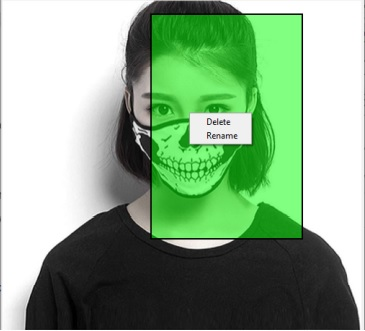
\includegraphics{images_latex/delate_rename.jpg}
\end{figure}
This will perform a simple rename of the tag for the current image and not a whole rename of a tag A in tag B (you can do it in Tag Panel).
To know the current annotation name, move the mouse on it and a little tooltip will display in the bottom-left corner of the annotator window.
Finaly, if you create a box that does not respect the parameter imposed (area size, sides lenght or covering constraints) a message error will be prompt to warn you about the impossibility of performing this task.
\subsection{The tag panel}

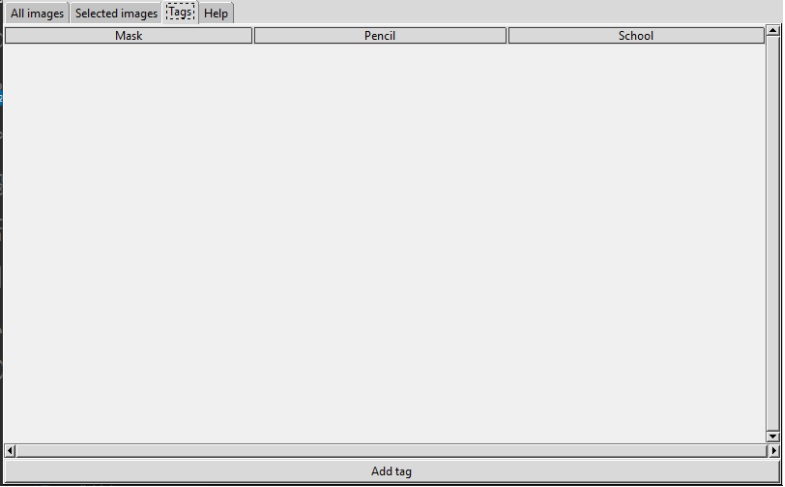
\includegraphics[scale=0.9]{images_latex/tag_panel.jpg}
This panel is composed of a grid of existing tags and an add tag button.

You can add a tag via the corresponding button and rename and delate an existing tag by clicking with the right-key of the mouse (in this case the rename will impact every image's annotation).
\subsection{The help panel}
The help panel contains a brief description of how our interface works and it is composed of four clickable buttons, each of them showing its related text. 
\subsection{Other features: the right panel}
\begin{wrapfigure}{r}{0.25\textwidth}
  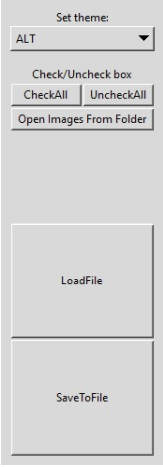
\includegraphics[scale=0.75]{images_latex/right_panel.jpg}
\end{wrapfigure}
The right panel of our interface contains some buttons performing different tasks.

You can modify the theme of the window via the OptionMenu under the \textit{"Set theme"} label (they are the default theme in case of \textit{"-fast"} execution of your OS or some customized themes in case of the \textit{"normal"} launch).

The other buttons:
\begin{itemize}
  \item checkAll: allow you to select every image of the \textit{"All images"} and pass them in the \textit{"Selected images"} panel.
  \item uncheckAll: that performthe inverse operation.
  \item Open Image From Folder: allows you to load the images of a custom folder.
  \item loadFile (resp.saveTofile): allows you to save (resp. load) a JSON file with the annotations of current (resp. previous) session.
\end{itemize}


\section{Conclusion}
In the first part of the project we created a functional interface to load and annotate images. We learnt how to use the tkinter library to correctly place tkinter objects and the shapely libraryto easly check area and converge of different shapes such as rectangular boxes.
The second part of the project, consists in

\end{document}